\documentclass[12pt]{article}
\usepackage[T1]{fontenc}
\usepackage[dvipsnames]{xcolor}
\usepackage{graphicx,amsmath,amsfonts,amssymb}
\usepackage{geometry}
\usepackage{tikz}

\title{Space domination}

\author{Cameron Jordan}
\date{}
\geometry{
	paper = a6paper
}
\begin{document}
\begin{titlepage}
\tikz[remember picture, overlay] \node[opacity=1,inner sep=0pt] at (current page.center){\includegraphics{coverimage.png}};
\begin{center}
\raisebox{30ex}{\colorbox{BurntOrange}{\huge{\textbf{\textsc{Space Domination}}}}}
\end{center}
\vfill

\colorbox{BurntOrange}{\textbf{Cameron Jordan}}
\thispagestyle{empty}
\end{titlepage}
\textcopyright CGJordan Publishing, 2025

Made using \LaTeXe
\vfill
\begin{center}
\includegraphics[scale=0.2]{logo.png}
\end{center}
\vfill

Components:
\begin{itemize}
\item Rule booklet
\item $3\times$ Starship
\item $9\times$ Torpedo
\end{itemize}
\thispagestyle{empty}
\newpage
\setcounter{page}{1}
\section*{The rules}

Play on the table top. 1 unit = 1 cm, adjust if needed. You can use rulers, meter sticks, tape measures or any other straight edge to represent vectors.

Each player's starship has 3 damage points. When a starship gets hit by a torpedo or another starship, it loses a damage point. If a starship reaches 0 damage points, flip it over and draw an `X' on the back. Should a starship's movement cause it to fly off the edge of the table the starship's damage points is reduced to 0.

Each player's starship starts with 3 torpedoes

Roll a six sided die to determine turn order, highest roll goes first. On your turn you can either move your starship or lauch a torpedo.

When your starship moves it accelerates in the direction it is pointing. Where your ship moves to is defined by a vector, $\vec{v}$, where:
\begin{equation}
\vec{v}=\vec{a}+\vec{r}\label{smoveq}
\end{equation}
calculated using the \textbf{tail to tip} method.

\underline{The \textbf{tail to tip} method}

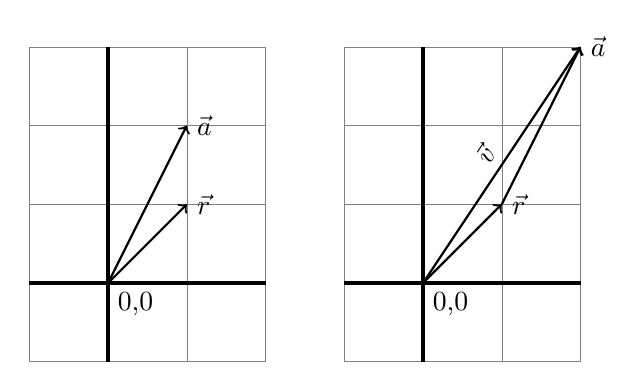
\begin{tikzpicture}
\draw[step=1cm, gray ,very thin] (-1,-1) grid (2,3);
\draw[very thick] (-1,0)--(2,0);
\draw[very thick] (0,-1)--(0,3);
\draw[->, thick] (0,0)--(1,1) node [anchor = west] {$\vec{r}$};
\draw[->, thick] (0,0)--(1,2) node [anchor = west] {$\vec{a}$};
\draw (0,0) node[anchor=north west] {0,0};

\draw[step=1cm, gray ,very thin] (3,-1) grid (6,3);
\draw[very thick] (3,0)--(6,0);
\draw[ very thick] (4,-1)--(4,3);
\draw[->, thick] (4,0)--(5,1) node [anchor = west] {$\vec{r}$};
\draw[->, thick] (5,1)--(6,3) node [anchor = west] {$\vec{a}$};
\draw[->, thick] (4,0)--(6,3) node [midway, sloped, above] {$\vec{v}$};
\draw (4,0) node[anchor=north west] {0,0};
\end{tikzpicture}

Given two vectors $\vec{a},\vec{r}$ adding them results in a new vector, $\vec{v}$. Note that two vectors that have the same magnitude and direction are equivalent no matter their position in the space.

When your ship moves it produces an acceleration vector, $\vec{a}$, with magnitude in units equal to the value rolled on a six-sided die that is in the direction of your ship's acceleration. When the game begins $\vec{r}=\vec{0}$, so on your first move $\vec{v}=\vec{a}$. On your turn before you move $\vec{r}$ is set to the $\vec{v}$ of the previous turn. On your next move you can accelerate again producing a new vector, $\vec{v}$ via eq.\ref{smoveq}.

While moving you may rotate your ship up to $180^\circ$ ($\pi$ radians) clockwise or counterclockwise.

When a torpedo is lauched the starship drifts along its $\vec{r}$. A topedo moves in the same fashion as a starship, but its initial direction is determined by the direction the launching starship is pointed, and the magnitude of the torpedo's $\vec{a}$ is always 6 units. A torpedo launched is not regained and only accelerates on the same turn as the starship it was launched from. At the end of its movement a torpedo always turns to face its target.\bigskip

\subsection*{Win condition} Be the last starship standing.
\newpage
\noindent\begin{tikzpicture}
\draw (0,0) node {\includegraphics[scale=1]{ship1bitmap.png}};
\draw (3,0) node {\includegraphics[scale=1]{ship2bitmap.png}};
\draw (0,-3) node {\includegraphics[scale=1]{ship3bitmap.png}};
%\draw (6,0) node {\textbf{Starships}};
%\draw (6,-1.75) node {\textbf{Torpedoes}};
\draw (3,-4) node {\includegraphics[scale=1]{torpedo1.png}};
\draw (4.5,-4) node {\includegraphics[scale=1]{torpedo1.png}};
\draw (3,-6) node {\includegraphics[scale=1]{torpedo1.png}};
\draw (3,-8) node {\includegraphics[scale=1]{torpedo1.png}};
\draw (4.5,-6) node {\includegraphics[scale=1]{torpedo1.png}};
\draw (4.5,-8) node {\includegraphics[scale=1]{torpedo1.png}};
\draw (0,-8) node {\includegraphics[scale=1]{torpedo1.png}};
\draw (1.5,-8) node {\includegraphics[scale=1]{torpedo1.png}};
\draw (1.5,-6) node {\includegraphics[scale=1]{torpedo1.png}};
\end{tikzpicture}\\\bigskip

\noindent\begin{tikzpicture}
\draw (0,0) node {\includegraphics[scale=1]{ship1bitmap.png}};
\draw (3,0) node {\includegraphics[scale=1]{ship2bitmap.png}};
\draw (0,-3) node {\includegraphics[scale=1]{ship3bitmap.png}};
%\draw (6,0) node {\textbf{Starships}};
%\draw (6,-1.75) node {\textbf{Torpedoes}};
\draw (3,-4) node {\includegraphics[scale=1]{torpedo1.png}};
\draw (4.5,-4) node {\includegraphics[scale=1]{torpedo1.png}};
\draw (3,-6) node {\includegraphics[scale=1]{torpedo1.png}};
\draw (3,-8) node {\includegraphics[scale=1]{torpedo1.png}};
\draw (4.5,-6) node {\includegraphics[scale=1]{torpedo1.png}};
\draw (4.5,-8) node {\includegraphics[scale=1]{torpedo1.png}};
\draw (0,-8) node {\includegraphics[scale=1]{torpedo1.png}};
\draw (1.5,-8) node {\includegraphics[scale=1]{torpedo1.png}};
\draw (1.5,-6) node {\includegraphics[scale=1]{torpedo1.png}};
\end{tikzpicture}
\end{document}